\documentclass[11pt, oneside]{article} 

\usepackage{geometry}                		% See geometry.pdf to learn the layout options. There are lots.
\geometry{letterpaper}                   		% ... or a4paper or a5paper or ... 

\usepackage[parfill]{parskip}    		% Activate to begin paragraphs with an empty line rather than an indent

\usepackage{fancyhdr}
\usepackage{textgreek}
\usepackage{hyperref}
\usepackage{graphicx}
\usepackage{mathtools}

\usepackage{ltablex}
\usepackage{multirow}
\usepackage{dcolumn}

\usepackage{lscape}
\usepackage{setspace}

\usepackage{color, colortbl}
\usepackage{array, booktabs, ragged2e}
\usepackage{makecell}
\usepackage{tikz}
\usepackage{textpos}


\usepackage{todonotes}


\definecolor{lightgray}{rgb}{0.83, 0.83, 0.83}

%\draftSpacing{1.5}

\pagestyle{fancy}
%\fancyhead{}

\title{Cattle, Cadaster, \& Conflict: \\ Settlement Growth and Social Conflict in Early Colonial New England 1620-1680}
\author{Eric H. Wilhelm %\\
%ECON 896
}
\date{}
\setlength{\parindent}{4em}
\setlength{\parskip}{0em}
\renewcommand{\baselinestretch}{2.0} 


\begin{document}

\maketitle

\begin{abstract}
\singlespacing
        Property rights are secure and violence over property is attenuated when the treatment and delineation of land are consistent, stable, and salient to each party. However, each party may have a different understanding about ownership over the same tract of land. How are divergent conceptions of ownership strained when one party (or group) is perceived as asymmetrically and rapidly accumulating property at another's expense? I examine the relationship between English settlement growth and the likelihood of conflict in 17th century colonial New England. Colonial growth halted when conflict erupted with surrounding Algonquian tribes during King Philip's War in 1676. One of the factors that spurred conflict was the perception (by Metacomet and the Wampanoag) of unanticipated, unchecked colonial growth. I use probate data covering 56 settlements in colonial New England to measure the growth of farmers as a proxy for territorial growth. After accounting for initial settlement size, English townships that doubled in farmer population were 10\% more likely to be damaged or destroyed during the conflict.     
 %Settlements within 20 miles of an Algonquian tribe were 53\% more likely to be damaged or destroyed. I also provide a qualitative summary of divergent perceptions among English settlers and Algonquian tribes leading up to conflict.
  \end{abstract}
\textit{JEL}: D23, D74, N41, O1, Q34, R14 \\
\textit{Keywords}: Political economy; Institutions; Property rights; Social conflict; Colonialism

\pagebreak

%Much has been said about the development of political and legal institutions as well as their impact on societal and economic outcomes (Acemoglu et al. 2001 \& Acemoglu, 2003). That literature used the era of European colonial expansion in Africa and the New World as a natural experiment to identify the types of colonial institutions installed around the world. Their experiment was to test whether the type of institution (i.e. the legal framework and form of governance) had any persistent effects on political stability and economic success. This trailblazing research broadly distinguished institutions as either ``extractive" in which property rights were not clearly enforced and where the state apparatus exploited indigenous resources and populations versus ``inclusive" in which settlers followed their home country's enforcement of property rights and form of self-governance (Acemoglu, 2003). The literature generally claims that colonies in North America (in what is today the United States and Canada) adopted the latter type of institutions (Cain \& Hopkins 1993). 

Institutions such as norms and rules define property rights and resolve property conflicts. They also reduce the likelihood and severity of violence over land. These institutions have been relegated to formal states %\todo{Any other \#statecapacity literature worth mentioning?} 
(Acemoglu \& Robinson, 2019; Johnson \& Koyama, 2017; and Dinecco \& Katz, 2016) or stateless channels of resolution (Candela \& Geloso, 2020). The violence-reducing characteristics of these institutions include: 1) defining property rights over space and time, 2) adjudicating contests over property, and 3) enforcing those resolutions after adjudication. Areas with little to no formal state institutions, such as the early colonial period in North America between European settlers and Algonquian Indians, mostly relied on the first characteristic. During the proceeding period of rapid colonial expansion during the mid-17th century, the mutually perceived definitions of land use between settlers and Algonquians changed. Rapid colonial population growth and expansion after the arrival of the {\em Mayflower} in New England made the process of defining and redefining property rights between Algonquian tribes and English settlers costly through peaceful means. The sharp change in relative growth (between the English and Algonquians) lowered the cost of violence compared to other, less violent appeals to trade or negotiation. 

This paper examines how rapid population growth relates to the likelihood and severity of violent conflict in areas without clearly defined property rights and areas without a mutually-agreed regime to resolve conflict over land. How did colonial expansion in New England confound the treatment of property rights between settlers and Algonquians?  Did rapid colonial expansion in New England mitigate or exacerbate conflict?  What was the relationship between early colonial expansion and the likelihood of conflict with Algonquians during King Philip's War?

The type of institution used to address and resolve potential conflict over land impacted the likelihood and severity of violence in colonial North America. The French colonial experience with Acadians and Mikmaqs in North America saw little to no conflict. The rules of collective decision-making for settling land disputes favored consensus and greatly reduced the returns to conflict (Candela \& Geloso, 2020). All parties had to come to a collective agreement which eschewed the formation of special interests who could potentially benefit from fighting, thus spilling the external costs of collateral damage onto the rest of the population. 

Initial settlements and competing interests over natural resources, such as the beaver, constrained the types of institutions that emerged in Canadian North America. European settlements around Hudson Bay had competing interests and varying property rights institutions. Native Americans in Fort Albany and York Factory faced competition in the beaver fur trade from the French (Carlos \& Lewis 1993, 1999, 2001). Hudson Bay Company managers increased the price of furs in those areas which led to more Native Americans to enter the market and deplete the beaver population more quickly. Fort Churchill did not face the same level of competition in the supply of beaver pelt. Prices for furs in that region were more stable, and the beaver population was not depleted as quickly (ibid).

Both colonial episodes in French Acadia and the Hudson Bay Company demonstrate how initial settlements, endowments, and incentives impacted the evolution of institutions that helped define property rights and resolve property conflicts. The types of institutions that evolved had varying success at mitigating violent conflict over land and managing natural resources. The colonial New England experience was characterized by an inchoate delineation of land use. New England also had higher colonist population growth in close proximity to Native Americans. In contrast to the French Acadia experience, colonial New England did not have an institution to resolve property conflict. New England also had a faster increase in settler population.

Recent empirical economic literature has looked at the reverse relationship between land conflict and contract choice in a modern context. %\todo{Let me know if you think this paragraph about modern-day impact is relevant/useful. I can drop it. I also don't know where to put it.}. 
Lee Alston and Bernardo Mueller (2010) analyze how land conflict and initial property endowments impact subsequent contract choice in Brazil. They use the extent of Catholic Church presence - measured by the number of priests - as an instrument for identifying the presence of farms without an official title. Their research looks at the impact of conflict on subsequent contract choice and the type of tenancy arrangement chosen. Similarly, Conning and Robinson (2007) examine how property insecurity impacts the type of agricultural organization selected among competing claimants. They use a model of potential land reform to demonstrate how an agent's expectations of property insecurity, instigated by the likelihood of land reform, are likely to modify their current choice of contract. Both papers measure the impact of property insecurity on subsequent contract choice.

%The story of colonial development in New England, however, was not free of conflict. 

After Jamestown was founded in 1607, early English settlements arose in the colonies of Plymouth and Massachusetts Bay. Pilgrims and later Puritan settlers - separatists of the Church of England - left Holland and England to escape religious-conformity restrictions imposed by the state religion of their home country. Disheartened by religious persecution, they wished to preserve their English identity and brought with them their own form of self-governance and legal framework (Winslow, 1646). The attitude of European colonizers towards {\em terra nullius} (``land with no owners") was varied (Pagden, 2015) and more ambiguous than their Dutch and French counterparts. 
%The General Court of Massachusetts decreed in 1648 ``that anyone who received a grant of land by what the court termed {\em vacuum domicilium} but did not build on or `improve' it within a space of three years would lose it" (ibid.). 
The land had to be tilled, sown, harvested, or grazed. A legal justification for agricultural development (a more land-intensive mode of food production) as well as a formal expression of property rights for English settlers in the Americas had been established.

The area of land spanning the coastline of Maine to Long Island Sound included many Algonquian peoples from the Massachusett around Massachusetts Bay, to the Wampanoag around Cape Cod Bay, and the Narragansett to the west in modern day Rhode Island (Washburn, 1989). Over the course of the 17th century, English settlers established various diplomatic, commercial, and religious connections with surrounding tribes, sachems (male leaders), and sunk-squaws (female leaders with great authority). Settlers and Natives conversed, intermarried, and formed treaties (Schultz, 1999 and Warren, 2018). 

They also exchanged goods and land. As the children and grand-children of England's first ``Great Migration'' came of age, by 1670 the English population burgeoned to over 60,000 people, almost double the Native New England population (Silverman, 2019). The population boom was not the direct source of conflict; nor was conflict {\em prior hoc} inevitable. Early interactions between Algonquians and the English (1620-1670) were pacific. What sparked tensions and, later, violent conflict was the rapid rise of English pastures and farms for husbandry - a dramatic increase in the demand for land. English settlers attempted to purchase land through various exchanges like manufactured goods or wampum, a string of beads used by Algonquian tribes as a form of currency (Brooks, 2018; Schultz, 1999). These trades often took a strategic tone in the greater context of internecine power relations among European powers and rival Algonquian tribes (ibid). The source of conflict resulted from poorly defined property rights - the perceived encroachment or illegitimate purchase of land between English settlers and the Wampanoag, Narragansett, and Nipmuck.

From the perspective of English settlers, an open expanse of land, a significantly depopulated Algonquian territory devastated by disease prior to the arrival of the English (Steckel et. al., 2002), and initial comity with the Wampanoag made the subject of contract choice relatively simple. Under consent and charter from the Crown\footnote{Sovereignty is not the same as individual right to property.}, most English requests for land were made through purchase (Pagden, 2015 and Roback, 1992). Challenges over occupancy with surrounding Native American tribes were generally met through treaty, gift, or exchange\footnote{Since their arrival, English settlers treated native land as {\em de facto} sovereign territory of American Indians. It would not be until the Treaty of Paris when the Royal Proclamation of 1763 formally ceded {\em de iure} autonomy to ``several Nations or Tribes of Indians".}. However, poorly defined property rights, ambiguous land-use arrangements between English settlers and Algonquian tribes, and rapid growth in settler population and land-intensive animal husbandry set the stage for one of the most devastating conflicts between the English and Algonquians in the Americas.

\section{Historical Background}

The Wampanoag, Narragansett, and Nipmuck settled in-land, away from the coastlines, and also along well-protected rivers and marshes (Washburn, 1989). Algonquian tribes had a deep knowledge of the terrain and exposed points of attack along coastlines where English colonists predominately settled. Generally, Algonquian forces were mobile and used their knowledge of the land to their advantage while the English typically fought in fixed points of defense near their settlements (Schultz, 1999). 

The introduction of livestock, expansion of land-intensive agriculture, and rapid settlement growth characterized early colonial development in New England. Four years after the arrival of the {\em Mayflower} in 1620, Edward Winslow, one of the early Pilgrim Fathers, brought from England ``three heifers and a bull, the first of any cattle of that kind in the land" (Anderson, 1994, p. 602). The task of improving the land was met as a general measurement of their prosperity. By 1627, Plymouth Colony had accumulated - either through husbandry or import - up to ``fifteen animals, whose muscle power increased agricultural productivity" (Anderson, 1979 \& PARP). In order to accommodate this land-intensive form of agriculture, Plymouth began expanding its borders beyond the boundaries of the compact village first established at the time of the first Thanksgiving. They traded manufactures and agricultural products with Massasoit, sachem of the Wampanoag and father of Metacomet, in exchange for more land.

The most lethal (and politically potent) of these manufactured goods were matchlock and flintlock firearms. The proliferation of guns was initially spurred by early colonizers (Silverman, 2016). Colonial governments were late to enforce the arms trade; and even when they began imposing restrictions on the movement of guns, black markets rose. The arms build up - predominantly spurred by Dutch, French, and English arms traders - revolutionized warfare for the Wampanoag. Metacomet, who the English called King Philip, saw the colonies as attempting to drive them off their land. Exacerbating tribal agitation, colonial governments banned the arms trade entirely and began confiscating arms from the Wampanoag (Lepore, 1998 and Silverman, 2016). The confiscation of arms and the perception of conquest came at a time of increased tensions between English colonists and the Wampanoag, Nipmuck, and Narragansett\footnote{The Narragansett remained neutral at the outset of King Philip's War and entered the conflict after peace negotiations with New England militias broke down.}. John Sassamon, a Wampanoag raised by an English family, was a mediator with significant influence in both societies. Harvard educated and a convert to Christianity, he also served as an advisor to Metacomet and was in the best position to ease the rising tensions. It was not until Sassamon was found dead in Assawompset Swamp in the winter of 1676 when conflict erupted. While the nature of Sassamon's death has never been confirmed, three of Metacomet's closest advisors were arrested, tried, and executed by Plymouth colonists for Sassamon's murder later that summer (ibid). Metacomet understood the colonists' summary judgement and execution as a threat. It meant the Wampanoag were a subject people and beholden to a foreign form of justice (Silverman, 2016). King Philip's War had begun.

\section{Theory}

Disagreements over land-use can either be resolved by jointly defining property rights in which both parties come to resolution; or the dispute could lead to violent conflict. In a setting with unclear property rights and no mutually-agreed authority to resolve disagreements over land-use, the likelihood of conflict is determined by the returns and costs to fighting. (See Figure 1). Returns to fighting over land are equal to the net present value of the land, natural resources, and strategic importance\footnote{For the purposes of the paper, the value of land is considered constant over time.}, $ R_{F} $, less the cost of fighting, $ C_{F} $.
$$ \Pi_{F} = R_{F} - C_{F} $$
Determinants for the cost of fighting in this historical context include the relative size of each population and relative level of technology (both in terms of weaponry and knowledge of the terrain). The relative values of each of those components are assumed to have constant returns to scale with respect to the cost of fighting such that $\alpha + \beta = 1$ and:
$$C_{F} =  \left[ \frac{N_{Colonists}}{N_{Algon}} \right]^{\alpha}  \left[ \frac{A_{Colonists}}{A_{Algon}} \right]^{\beta}$$
Where N is population and A is military technology. Assuming the relative technologies of each group stays the same and the population of American Indians holds constant over time, the change in the cost of fighting will mostly be determined by the change in the population of colonists such that:
$$ \frac{\delta N_{Colonists}}{\delta N_{Algon}} > 1$$
This framework assumes the likelihood of conflict has a direct relationship with the relative cost of fighting. All else constant, including the returns to fighting, did the relative change in growth of the English settler population result in a lower cost to fighting? 
%The cost of fighting in the context of mid-17th century colonial New England was mostly determined by the relative expansion in settler population.
\\

\begin{figure}
\caption{Returns to Fighting}
  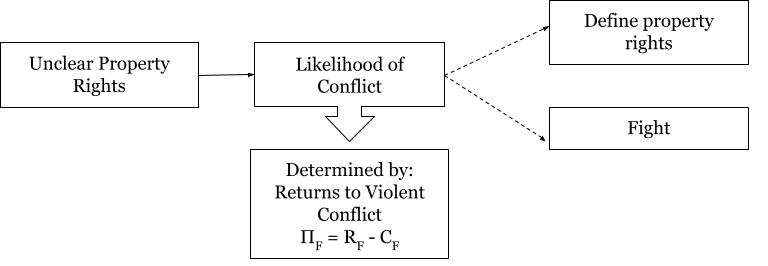
\includegraphics[scale=.65]{TheoryGraph.jpg} 
\end{figure}

%In the late nineteenth century, anthropologists and sociologists held a pervading belief that all property (including land) in hunter-gatherer societies was collectively shared (ibid.). Speck (1915) later challenged that notion with evidence linking group ownership to specific tracts of land among Native American peoples in northeastern North America. Contrary to the early historical notion of shared collective lands, hunter-gatherers in this region were found to be territorial, rigid, and responsive to intrusions on their property. ``Transgression of their boundaries often resulted in deadly struggle" (Baker, 2003).

\noindent\textbf{Hunter-Gatherer Land Tenure Model}

In order to model the stylized facts of rapid colonial expansion and subsequent conflict with surrounding Algonquian tribes, I rely on Baker's model of land tenure and conflict for hunter-gatherer societies (2003). Baker makes general assumptions about ecological parameters, resource density, resource predictability (the change in harvest of game or crops over time), and situational ownership to develop a contest-success function that models predictions about ownership changes, investment in defensive technologies, and land tenure regimes (2003). 

%Contributing to previous work on the theory of conflict from Hirshleifer (1995), Baker incorporates additional parameters into this two-player, multi-period model that endogenizes the size of the object being contested (land) which influences the marginal benefits and costs associated with investing in defense and intrusion technologies. After presenting Baker's initial assumptions and resolving the model's first proposition about territorial exclusivity, I reference the model's optimal strategies \footnote{Derived from backwards induction of payoffs and first order conditions.} and repurpose them to identify the breaking point when English settlement growth would instigate conflict.

\begin{figure}
%Figure here.
\caption{Depiction of Land Tenure and Conflict}
  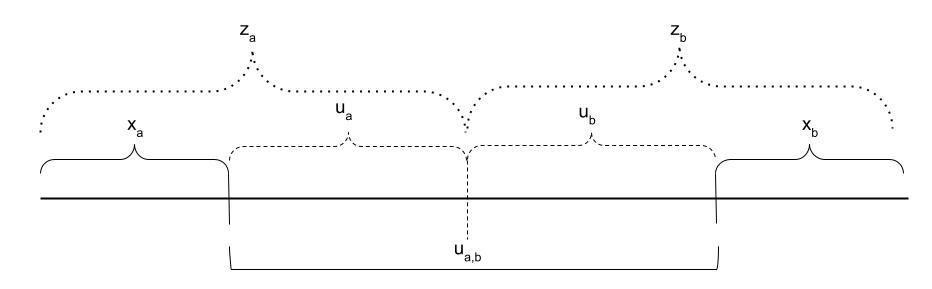
\includegraphics[scale=.5]{LandConflict.jpg} 
%\begin{figurenotes}
%Figure notes without optional leadin.
%\end{figurenotes}
%\begin{figurenotes}[Source]
%\\
%Depiction of Land Tenure and Conflict
%\\
%Source: Baker, 2003
%\end{figurenotes}
\end{figure}

The adapted contest-success model is laid out as follows:

\begin{enumerate}
\item Fixed amount of land, $z$
\begin{itemize}
\item Each player, $a$ and $b$, is endowed a certain amount of land, $z_a$ and $z_b$, respectively
\item The two players exhaustively lay claim to all contested land such that $z=z_a+z_b$
\item Average density of resources
\item Each fixed unit of land yields a predictable output
%\item Combined ``quality of land" measure is denoted, $\delta$
%\item Each player knows the ecological parameters but the resource level is not realized
\end{itemize}
\item Each player has an assigned production technology and preferred value of the land
\item Players decide how much land to defend, $x_i$
\item Any uncertainty with respect to how much land $x_i$ is apportioned to whom is due to undefined or unrecognized property rights
\item Each player invests in defensive, $d_i$, \& offensive, $g_i$, capabilities  
\item  Groups observe the amount and quality of land the other groups have defended as well as their defensive investments
\begin{itemize}
\item Groups make intrusive/offensive investments to gain access to undefended, $u_i$, and then defended, $d_i$, territories of the other group
\end{itemize}
\item Simultaneous intrusive investments on land left undefended
\item Groups receive payoffs according to the outcomes of the interaction between each group's offensive and defensive investments. Random variables related to the resource level are realized. The model allows for entry and exit after the first round of play.
\end{enumerate}

\noindent Figure 2 illustrates the relationships between these variables - endowment $z_i$, defended land $x_i$, undefended land $u_i$, as well as defensive investment $d_i$ and intrusive investment $g_i$. Each player elects to defend some subsection of their endowed parcel of land, $x < z$. A marginal cost attributable to defensive and intrusive capabilities such as weapon technology, ``fighting ability, policing, marking boundaries [cadaster], and negotiation" is assumed to be constant and identical for both groups, $c$ (ibid.).


Putting all of these pieces together, the share of endowed land that defending groups choose to defend ($x_i$) - indicative of the relative cost of fighting for group $i$ - is given by:
\begin{equation}
f_i(d_i, g_j)=\frac{1}{1+(\phi g_j/d_i)},\; \; i=a,b;\, j=b,a.
\end{equation}

\noindent Where $\phi \in (0,1) $ is a constant parameter of the relative strength of $j`s$ offensive capability relative to $i`s$ defensive capability. Specifically, I am estimating the relationship between colonial population growth $g_{j}$ on the cost of fighting $f_i(d_i, g_j)$ which is proxied as the likelihood and severity of conflict in a colonial settlement.
%\noindent The model incorporates spatial features that assumes increased difficulty in the defense of land that increases with size. The function $\phi$ depends on the size of the defended territory and assumes the relationship is linear:
%\begin{equation}
%\phi(x_i) = \phi_0 + \phi_1 x, \; \; \phi_0>0,\, \phi_1>0.
%\end{equation}
%\noindent Following a Stackelburg structure in which the defender has the first move, the optimal strategy is solved through backwards induction beginning with the intrusive investment decisions for each group. Starting with the intrusive investment decision for group $j$ in Step 5, Baker maximizes the share function with respect to $g_j$. The same optimality condition is determined from the perspective of the opponent's defensive investment - maximizing the share function with respect to $d_i$ - to determine the optimal choice of defense.

%After identifying the optimal intrusive and defensive strategies for each player, Baker obtains Proposition 1 which provides the conditions under which a defending group chooses an optimal defense $d$:

%\newtheorem{prop}{Proposition}

%\begin{prop}
%(1) If $\frac{1}{2} \geq \phi(x_i)$, then $d^*_i=d^0$, $g^*_j=0$, and $s_i=1$, $i, j = a, b$. (2) If $\frac{1}{2} < \phi(x_i)$ then,

%\begin{equation}
%d^*_i = \frac{\alpha\delta x_i}{4\phi(x_i)c},
%\end{equation}
%\begin{equation}
%g^*_i = \frac{\alpha\delta x_i}{2\phi(x_i)c} \left[ 1 - \frac{1}{2\phi(x_i)} \right],
%\end{equation}
%\begin{equation}
%s_i=\frac{1}{2\phi(x_i)}.
%\end{equation}

%\end{prop}

%The first part of Proposition 1, (1) implies that smaller territories are more likely to be exclusive, less prone to intrusion by the opponent, and geographically stable. Assumption (2) lists the optimal defending and intruding strategies when the territories are no longer exclusive and prone to conflict - when territories are of size $\frac{1}{2}<\phi_0 + \phi_1 x$. The point in which defended territory is no longer \textit{exclusive}, $x^0$, is defined as $\frac{1}{2}=\phi_0 + \phi_1 x$. Solving for $x^0$ gives:
%\[
%x^0 = \frac{1-2\phi_0}{2\phi_1}
%\]

%This equality identifies the point in which a group's territory is not exclusive and can be intruded upon. For my purposes, I stop here and begin modulating the optimality conditions \footnote{The rest of Baker's paper builds upon the net value and cost of the defended land to model the various land tenure regimes (e.g. Geographically Stable, Spatio-Temporal, and Spatio-Temporal Territories with Open Access) that change relative to changes in ecological conditions, defensive technologies, and land-value preferences.}. For purposes of this paper, I rely on the optimal strategies derived from the first order conditions after the first round of play to identify the likelihood of conflict in a \textit{non-exclusive} or contestable territory.

%My incremental innovation is to maximize the optimal share of contested land [see: Proposition 1, Assumption (2)] held by the defender (English settlers) relative to the amount of land defended, $x_i$, subject to the optimal intrusive investment strategy (of Algonquian tribes), $g_j$, less the optimal defensive investment strategy (of the English), $d_i$. What is the maximum share of contested land that the defender can hold assuming each player plays the optimal intruding/defending strategy?
%\[
%Max share of contested endowed land with respect to land defended constrained by optimal defending/intruding strategies
%\max_{x_i}  s_i - \left[ g^*_j - d^*_i \right], \; \; \, g^*_j \geq d^*_i
%\]
%I assume the breaking point for conflict is when the optimal investment in intrusion for player $j$ exceeds the optimal investment in defense for player $i$. Substituting equations (3) - (5), differentiating with respect to $x_i$, and solving for $x_i$, I find:
%\begin{equation}
%x_i \leq \frac{\phi}{\phi^{'}} - \frac{2c}{\alpha\delta(1-2c)}
%\end{equation}
%Rewritten in terms of the \textit{growth rate} of defended territory, $\frac{\phi^{'}}{\phi}$, and setting the marginal cost of ``property rights enforcement technology" $c=1$ for simplicity, the breaking point (when $j$ intrudes) occurs when the growth rate of $i$'s defended territory meets the following inequality:
%\begin{equation}
%\frac{\phi^{'}}{\phi} \geq \frac{1}{x_i - (\frac{2}{\alpha\delta})} \tag{***}
%\end{equation}

%Similarly, the richer the value of land being contested, a higher $\alpha$ or $\delta$, the smaller the growth rate required to induce conflict. Determining values for resource value, density, predictability, and other measures of land quality, as well as testing their impact on the likelihood of conflict will be attempted in future research. The following empirical analysis identifies the naive relationship between settlement growth rate and likelihood of conflict. 

A settlement with a larger initial defended territory, $x_i$ (or initial settlement), requires a lower subsequent population growth rate to induce conflict. I later test this relationship controlling for initial settlement size. The value of the land being defended may be more intersubjective and dependent on the perceptions held by Algonquian tribes and English settlements. The initial settlement size is also subject to intergenerational perceptions across both groups of people. In conjunction with the narrative summary in Appendix A, (see ``Interactions Prior to King Philip's War'' Table in Appendix A), I relay various sources of interactions prior to conflict that either exacerbated or dampened the relationship between colonial growth and the likelihood of conflict.

\section{Macro Analysis}
From the perspective of Algonquian tribe, $i$, the model describes how changes in a nearby\footnote{Within $z$ distance from $i$} English settler population, $g_j$, impacts the cost of fighting, $f(\cdot)$ (Equation 1) as observed through the likelihood of fighting. An increase in $g_j$, all else constant, would decrease the cost (and increase the likelihood) of fighting.
%One of the motivating factors for conflict was the perception of rapid settlement expansion. 
In an attempt to measure the magnitude of the expansion, I examine the relationship between the rate of colonial expansion and the likelihood of conflict at the township level. I first quantify the magnitude of early colonial expansion across all settlements in colonial New England and identify whether that township was damaged or destroyed during King Philip's War. I projected estimates of the likelihood of conflict using a logistic {\em LOGIT} regression which is typically used for identifying the relationship of a binary outcome variable - the probability of a town being damaged or destroyed. Descriptions of the models, data, and results are below.

\noindent\textbf{Models}

A first-best measurement of colonial expansion would be the change in land area of each township over the preceding decades. Growth in settlement area would propagate interaction between the English and surrounding tribes, and according to the contest-success function model's hypothesis, increase the likelihood of conflict. Unfortunately, data on cadastral \footnote{The formal surveying and public assignment of cadasters do not begin historically until later in the 17th century. Throughout this paper, I use the term ``cadaster" simply as a publicly salient delineation of property.} size and development for each township is not available at the macro level. Instead, I use the growth rate in the population of farmers since the decade of initial founding as a proxy for land growth over the same time period.
The following model is used to illustrate the relationship between colonial expansion and the likelihood of conflict:
%\pagebreak
%\[(1) \ TownDamaged_{i} = \beta_0*FarmerGrowth_{i} + \epsilon 
%\]
%\[
%(2) \ TownDamaged_{i} = \beta_0*FarmerGrowth_{i} + \beta_1*InitFarmerPop_{i} + \epsilon
%\]
%\[
%(3) \ TownDamaged_{i} = \beta_0*FarmerGrowth_{i} + \beta_1*InitFarmerPop_{i} + \beta_3*Win20MI_{i} + \epsilon
%\]
%\[
%(4) \ \ \ \ TownDamaged_{i} = \beta_0*FarmerGrowth_{i}*WGT_{InitFarmerPop_{i}} + \epsilon
%\]
\[ (1) \ \ \ Log(TownDamaged_{i}) = a + \beta_0*FarmerGrowth_{i}*WGT_{InitFarmerPop_{i}} + \epsilon
\]
\noindent Where and $WGT_{InitFarmerPop_{i}}$ is the population upon initial settlement.
%\\
%Coefficient ``\textbf{a}" represents a constant - or baseline likelihood of conflict - for a township residing in any New England colony at the steady state. The \textbeta \ coefficient represents the incremental impact of township growth on the likelihood conflict.
%\bigskip

\noindent\textbf{Data}

%\todo{Lewis (2004), other papers that relate population growth to land use.} 
The data for farmer population and real estate value come from a sample of colonial New England probate records from 1620 to 1675 (Main, Main \& Lindert, 2013). The universe covers all deceased individuals - including landowners and landless tenants - in southern New England over this time period. The probate data also include categories for each individual's occupation, value of real property, wealth \footnote{Wealth measurements include real property as well as other types of capital.}, debt, age, and sample weight by age group \footnote{The weight equals the inverse of the probability of selection for a deceased individual of a certain age group reported in the sample. For example, a deceased individual is more likely to be older than younger. The probability of a sample probate listing an older person is higher than a younger person.}.

% \footnote{The universe excludes what are today New Hampshire and Maine.}
%\footnote{Various measurements for the value of real property are reported in sterling, real sterling, and dollar equivalents. I used the value for real sterling in this analysis and was able to crosscheck those values using the nominal figures and deflator they provided.}

%One point of concern between the stated variable of interest (i.e. land) and the data available in the sample (i.e. farmer population and value of real estate) is a discrepancy in the data generating process for each variable. 

The size of a township cadaster is a {\em stock} measurement of land; the number of deceased individuals reported in the probate is a {\em flow} measurement of the colonial population. %\todo{I need to investigate demography papers that address measurements of pop growth given limited data. I have (naturally lagged) probate data.}. 
To account for this discrepancy, I aggregated the farmer population\footnote{Each record represents a deceased individual. The farmer population of a given township equals the sum of the sample weights across all individuals listed as a farmer, artisan-farmer, or laborer. See: Occupational codes listed in the probate codebook.} by decade.

%The assumptions here are twofold:  1) an aggregate flow of deceased individuals over the course of a decade is a close approximation to the stock of farmers or land held by a township at a specific time period and 2) a decade-over-decade growth rate is a close approximation to a change in the stock of land.

The benefit of aggregating probate records by decade comes at the cost of fewer observations and less variation. Annualized growth rates had many gaps, were too variable, carried too much noise, and did not reasonably represent changes in the stock of colonized land. The model assigns one decennial growth rate to each township, {\em i}. The decennial growth rates were computed using a straight-line approach:
\[
Decennial \ Growth \ Rate \ =
\]
\[
\frac{ 1670 \ to \ 1676 \ Total - First \ Settlement \ Decade \ Total }{First \ Settlement \ Decade \ Total} *
\frac{100}{Number \ of \ Decades}
\]
%\\
I consider the measurement of farmer population to be more economically representative of land growth relative to real estate value. Seventeenth century frontier farming in the American Colonies is best described as a factor minimizing production function between land (capital) and labor: $F(K,N)=min[K,N]$. This type of production function treats land and labor as complements. It assumes that a given acre of land cannot yield more output (or be anymore productive) by substituting towards more labor. Given that assumption, any increase in agricultural production would need to be met with a one-to-one increase in {\em both} factors. 
%\todo{Descriptive Stats of Probate Data: Number of townships, aggregate population count by year and decade}

Figure 3 in Appendix A highlights in red or yellow each of the townships that were damaged or destroyed during King Philip's War. The source for township damage comes from a collection of accounts from the war portrayed in Figure 1, Appendix A (American History Online). For this analysis, I assigned a binary variable of 1 to any township that was either damaged or destroyed during the war. Although the map distinguishes between destroyed and damaged towns, the relative magnitude of destruction is unknown. I consider any sign of war-related property damage as sufficient for indicating conflict. Figure 7 in Appendix A is a magnified map showing tribal settlements in yellow and ``Indian praying towns'' (Christian missions) in black. 
\pagebreak

\noindent\textbf{Results}

%\todo{Update LOGIT model. Include PROBIT model. Update table of results after making changes} 
Table 1 shows the estimates and standard errors for models (1) through (5)\footnote{I had originally limited the analysis to Hampshire and Plymouth counties where the fighting occurred. Increasing the coverage to span all colonial New England townships dampened the effect but increased precision.}. The dependent variable of interest is a binary indicator of a town being damaged or destroyed during King Philip's War. A $LOGIT$ model accounts for this binary relationship and bounds the predicted values to between zero and one. Model (5) is a logistic regression measuring the relationship between the population growth rate with the likelihood of the township being damaged or destroyed. Rewriting equation (5) with the parameters in column (5) of Table 1, the relationship between farmer population growth and the likelihood of conflict can be expressed:
\[
P(TownDamaged_{i})=\frac{1}{1+e^{2.37-0.09*GrowthRate_{i}}}
\]
According to Model (5), a settlement that doubled in size over the period of initial settlement to 1670 was 10\% more likely to be damaged or destroyed during King Philip's War. %\todo{Can I measure severity of conflict that weighs destroyed settlements more than damaged settlements?} 
Townships with higher growth rates \textit{decrease} the denominator which \textit{increases} the probability of a town being damaged or destroyed. Future testing will include additional parameters such as other distances to the nearest tribal settlement, measures of resource value, and investment in defense. 

%Models (1) and (2) report a coefficient of 0.009 and 0.008. Both coefficients are statistically significant at a 5\% level of confidence. These coefficients indicate that a decennial growth rate of 100\% in the population of farmers (i.e. doubling since first settlement) corresponds to a 0.9 or 0.8\% increase in the likelihood of conflict. Given that farmer populations grew by a factor of 2 to more than 20 for some townships over this time period, the magnitude of this result is descriptively meaningful. The coefficients for growth are about the same for both sets of results.

%Figure 2 shows the scatter plot, linear representation, and initial settlement population for model (1). The OLS model is bounded between 0 and 100\% for all observations. A coefficient of 0.09 suggests that colonial New England townships that doubled in size were just under 1\% likely to be damaged during King Philip's War. As a close approximation, each factor increase in settlement size corresponded to a one percentage point increase in the likelihood of conflict. Figure 3 limits the number of townships in Figure 2 to towns that grew less than a factor of 20, about 2 standard deviations above the mean growth rate observed across all New England townships. The slope does not change significantly after removing outliers.

%Model (3) is an OLS representation of three variables considered in the contest-success functions described in Section 2:  growth, population, and proximity (to rival). In that model, proximity to the nearest tribal settlement sharply increases a township's likelihood of being damaged by 53\%. The effects of farmer growth and initial farmer population fall to zero. The overall descriptive power of model (3), as measured by Adjusted $R^2$, increases substantially. This is the only model that achieves an F-statistic greater than 10. Given the likelihood of conflict is operating on the margins of growth (rapid expansion) and proximity (distance to nearest tribal settlement), future testing that modulates the distance from the nearest tribal settlement may provide more insight.

%\pagebreak 

\begin{landscape}

\begin{table}[!htbp] \centering 
\resizebox{.78\textwidth}{!}{\begin{minipage}{\textwidth}
  \caption{Model Results} 
  \label{} 
    \hskip-5.5cm
\begin{tabular}{@{\extracolsep{5pt}}lD{.}{.}{-3} D{.}{.}{-3} D{.}{.}{-3} D{.}{.}{-3} D{.}{.}{-3} } 
\\[-1.8ex]\hline 
\hline \\[-1.8ex] 
% & \multicolumn{5}{c}{\textit{Dependent variable:}} \\ 
%\cline{2-6} 
\\[-1.8ex] & \multicolumn{5}{c}{Town Damaged} \\ 
\\[-1.8ex] & \multicolumn{4}{c}{\textit{OLS}} & \multicolumn{1}{c}{\textit{Logistic}} \\ 
\\[-1.8ex] & \multicolumn{1}{c}{(1)} & \multicolumn{1}{c}{(2)} & \multicolumn{1}{c}{(3)} & \multicolumn{1}{c}{(4)} & \multicolumn{1}{c}{(5)}\\ 
\hline \\[-1.8ex] 
 Farmer Growth & 0.009^{**} & 0.008^{**} & 0.004 & 0.022^{**} & 0.091^{***} \\ 
  & (0.003) & (0.003) & (0.003) & (0.009) & (0.025) \\ 
  & & & & & \\ 
Initial Farmer Population (Hundreds) &  & 0.003 & -0.001 &  &  \\ 
  &  & (0.002) & (0.002) &  &  \\ 
  & & & & & \\ 
 W/in 20 miles of Indian Settlement &  &  & 0.532^{***} &  &  \\ 
  &  &  & (0.102) &  &  \\ 
  & & & & & \\ 
 Constant &  &  &  &  & -2.371^{***} \\ 
  &  &  &  &  & (0.147) \\ 
  & & & & & \\ 
\hline \\[-1.8ex] 
Observations & \multicolumn{1}{c}{56} & \multicolumn{1}{c}{56} & \multicolumn{1}{c}{56} & \multicolumn{1}{c}{56} & \multicolumn{1}{c}{56} \\ 
R$^{2}$ & \multicolumn{1}{c}{0.108} & \multicolumn{1}{c}{0.131} & \multicolumn{1}{c}{0.425} & \multicolumn{1}{c}{0.104} &  \\ 
Adjusted R$^{2}$ & \multicolumn{1}{c}{0.091} & \multicolumn{1}{c}{0.098} & \multicolumn{1}{c}{0.393} & \multicolumn{1}{c}{0.088} &  \\ 
Log Likelihood &  &  &  &  & \multicolumn{1}{c}{-235.442} \\ 
Akaike Inf. Crit. &  &  &  &  & \multicolumn{1}{c}{474.884} \\ 
Residual Std. Error & \multicolumn{1}{c}{0.337 (df = 55)} & \multicolumn{1}{c}{0.336 (df = 54)} & \multicolumn{1}{c}{0.276 (df = 53)} & \multicolumn{1}{c}{1.118 (df = 55)} &  \\ 
F Statistic & \multicolumn{1}{c}{6.636$^{**}$ (df = 1; 55)} & \multicolumn{1}{c}{4.053$^{**}$ (df = 2; 54)} & \multicolumn{1}{c}{13.067$^{***}$ (df = 3; 53)} & \multicolumn{1}{c}{6.373$^{**}$ (df = 1; 55)} &  \\ 
\hline 
\hline \\[-1.8ex] 
\textit{Note:}  & \multicolumn{5}{r}{$^{*}$p$<$0.1; $^{**}$p$<$0.05; $^{***}$p$<$0.01} \\ 
\end{tabular} 
 \end{minipage}}
\end{table} 

\end{landscape}

%\pagebreak

%Model (4) is an OLS representation of model (1) after weighting each township's growth rate with the size of their initial farmer population in the decade of their first settlement. Townships with a larger initial farmer population are weighed more heavily than townships with a smaller initial population. This approach accounts for the mathematical reality that a settlement with a smaller population baseline can achieve a much higher growth rate than a settlement that began with a much higher population\footnote{Interactions among growth rates, initial settlement size, and proximity to tribal rivals will be tested in future research.}. 

%The coefficient for growth (weighed by initial settlement size) in model (4) is twice as large as the coefficients in naive models (1) and (2). This suggests a confirmation of the prediction in Section 2 that a lower growth rate is required to induce conflict for larger (initial) settlements. A larger coefficient in model (4) suggests that the same growth rate (which was equally weighted) in model (1) would be more likely to induce conflict after attributing a higher weight for larger initial settlements. The multiplicative relationship between initial settlement size and subsequent growth derived from Section 2 is better represented in model (4) than models (1) and (2).

%A similar \textbeta \ coefficient is observed for model (2) which uses decennial growth in the value of real estate as the explanatory variable. However, this result is not statistically significant. Like model (1), a doubling of the value of real estate decade-over-decade corresponds to an increase in the likelihood of conflict by 5\%. Figure 3 in Appendix B shows the scatter plot, linear representation, and OLS equation for model (2). The intercept is much higher at 47\%. The results of this model appear to pull all of the values upwards along the probability-of-conflict axis \footnote{This is predominately an artifact of the exclusion of townships along Cape Cod.} relative to model (1). As noted earlier, the growth in real estate value is not as representative of land growth as the growth in farmer population. However, the descriptive coefficient for each proxy variable tells a similar story. Townships that grew at a faster clip were more likely to face damage over the course of the war.

%Table 2 reports estimates for the impact of  growth in real estate value on the likelihood of conflict. Those results include townships in Cape Cod which were some the earliest English settlements in the region. Cape Cod settlements were also located along the coastline and geographically distant from any Wampanoag village. The conflict estimates derived from the growth in real estate value (both weighted and unweighted) are neither meaningful nor significant. 

\section{Micro Analysis}
The macro analysis suffers from an absence of data on the growth of land in English settlements, measured in terms of surface area (e.g. acres or hectares). In order to corroborate the magnitude of the growth rates observed in the macro analysis (which solely relied on the population of farmers that entered probate), I also looked at archaeological data on livestock (and pasture size) over the same time period for Plymouth township to see whether the growth in livestock reconciles with the proxy variables used in the macro analysis. Using United States Department of Agriculture (USDA) guidance on pasture size capacity, I imputed the total number of pasture acres required to accommodate the number of livestock reported in the archaeological site.

\noindent\textbf{Plymouth Archaeological Rediscovery Project}

Craig Chartier and other members of the Plymouth Archaeological Rediscovery Project used faunal analysis to catalogue and substantiate the number of cattle reported in select probate records across three sites within Plymouth township (Chartier, PARP). The faunal results reported in Figure 5 of Appendix A show the total stock of cattle for each decade. Ratios of other types of livestock relative to each cow were also confirmed in the archaeological analysis. I applied those ratios to the total stock of cattle to derive the total number of livestock for each decade. The total number of livestock and decennial growth rate in the number of livestock are reported in the last two columns of the lower table in Figure 5.
\\

\noindent\textbf{Pasture Size}

Using the USDA formula, I then imputed the pasture size required to accommodate the livestock reported in Figure 5. The USDA formula is adapted for small-scale farm use and mixed operations including foraging and crop rotation (NRCS, USDA). These assumptions are more relevant for 17th century agriculture and English farming methods. I scaled down the average size of each animal (assuming scrawnier 17th century livestock) as well as reduced the utilization rate and average yield per acre to reflect a level of farm productivity that is closer to subsistence. For the purpose of this analysis, an accurate estimate of absolute land size is not as important as the decennial growth rate. The growth rate is entirely driven by the growth in cattle reported from archaeological evidence and the ratios of livestock weight.

The total number of acres required to house each type of livestock are reported by decade in Figure 6. The assumptions I made for average livestock weight, utilization rate, grazing days per year, and average yield per acre are listed on the top left. The pasture size imputations reported in Figure 6 are constructed using the USDA formula and total livestock figures reported in Figure 5. The decennial growth rate in pasture size for Plymouth township is reported in column 7 of Figure 6. The highlighted records in Figure 6 compare the decennial growth rates of the micro analysis to the growth in farmer population and real estate value reported for Plymouth derived from the probate records used in the macro analysis. The growth rates show a similar pattern:  a rapid expansion in 1630-1640, moderate growth in 1650-1660, followed by a decline resulting from King Philip's War in the later part of the 1670's.

\section{Additional Tests and Future Research}

\begin{itemize}
%\item Read the literature on Hunter-Gatherer Land Tenure - the debate about whether hunter-gatherer societies collectively owned land
%\item Read about Man the Hunter conference and legacy debate on land ownership in ancient hunter-gatherer societies
%\item{Run models (1) and (2) using a pentennial (five-year) growth rate}
%\item Measures of ecological parameters such as soil suitability, terrain ruggedness, and average rainfall
%\item{Research missionary records to identify ``praying towns" - areas where English farming methods and religious tenants were shared with Native Americans.} 
%\item{Run a {\em Logit} regression on levels of real estate value (and farmer population) by year}
%\item{Run a {\em Probit} regression on levels of real estate value (and farmer population) by year}
%\item{Impute the levels of real estate value} 
%\item Impute farmer populations for townships with missing data using other available data in the probate records
%\item Use a p-score method to extrapolate relationships between other probate variables (e.g. real estate value, wealth, debt, occupation) from other surrounding towns
%\item{Apply the annualized growth rate observed for the entire time span of that township to the previous year}
%\item{Run a {\em Logit} regression with those imputed values}
\item{Research demography literature on population growth accounting with incomplete, lagged probate data}
\item{Test colony/county-wide fixed effects, e.g. First settlement date during Republican Period?}
%\item{ {\bf Consider the impact of Crown disinterest during the {\em Glorious Revolution} }} 

%\item{Find/add more quantitative \& qualitative descriptors for each township}
%\begin{itemize}
%\item{Delineate colonial diplomatic relations with surrounding Algonquian tribes and other European colonizers nearby. i.e. Dutch \& French}
%\item{Measure the extent of social interaction and trade between each township and surrounding tribes}
%\end{itemize}
\item{Replace map of conflict areas with Washburn Handbook of North American Indians. Other data sources for areas of conflict? Krech?}
\item{Provide summary statistics of probate data}
\item{Run revised LOGIT model and include PROBIT model.} 
%Is it OK to include more than one parameter in a LOGIT/PROBIT model? I'm not sure how to interpret the results of a multivariate LOGIT/PROBIT model.
\item{Collect ArcGIS information on soil fertility, amount of precipitation, and other time invariant geographical information on quality of land}
\item{Consider instruments or other proxy variables for land growth / ``potential for land confrontation"}

%\begin{itemize}
%\item{How did Native Americans interact with Puritan missionaries?}
%\item{What palliative role did "praying Indians" have when mediating between English settlers and Algonquian tribes? e.g. John Sassamon }
%\end{itemize}

%\item{Identify the form of government and treatment of property for each Algonquian tribe}
%\item{Map inter-tribal rivalries and alliances}

\end{itemize}

\section{Conclusion}
Many factors contributed to the onset of King Philip's War:  colonial expansion, disparate treatment of property, the proliferation of guns, inter-colonial and inter-tribal rivalries, and - as is the case for every conflict - the failure of diplomacy. It was clear that property rights enforcement and the perception of justified expansion were not shared between English settlers and Algonquian tribes. But the absence of shared property enforcement does not inevitably lead to conflict. 
%Perhaps the New England frontier was a {\em terra nullius} or Hobbesian ``state of nature". Those arguments, however, were used to justify the colonization and expansion of English settlement, not propose a common approach to property with Native Americans.

Colonial growth in New England was very significant and geographically heterogenous in early to mid 17th century. Townships grew by as small as a factor of 2 to as high as a factor of 20. Threats such as weapons confiscation and perceived loss of land drove the Wampanoag and other Algonquian tribes to violence. After accounting for proximity to the nearest surrounding Algonquian tribal settlement, townships that grew more rapidly during the early stages of colonization were more likely to be targeted during the war. 
%Larger initial settlements were more likely to induce conflict with relatively lower subsequent growth rates.

\pagebreak

\begin{thebibliography}{1}

%\bibitem{acem} Acemoglu, Daron. ``Why not a political Coase theorem?  Social conflict, commitment, and politics."  {\em Journal of Comparative Economics}. Vol. 31, Issue 4. (September 2003). pp. 620-652.
%\smallskip
\bibitem{acemr} Acemoglu, Daron, and James A. Robinson. {\em The Narrow Corridor: States, Societies, and the Fate of Liberty}. Penguin Press. New York, NY. (2019).
\smallskip
%\bibitem{acemo} Acemoglu, Daron, Simon Johnson, and James A. Robinson. ``The Colonial Origins of Comparative Development:  An Empirical Investigation."  {\em American Economic Review}. Vol. 91, No. 5. (December 2001). pp. 1369-1401.
%\smallskip
\bibitem{alston} Alston, Lee J. and Bernardo Mueller. ``Property Rights, Land Conflict, and Tenancy in Brazil."  {\em National Bureau of Economic Research}. Working Paper 15771. (March 2010).
\smallskip
\bibitem{amer} American History Online. ``King Philip's War."  Accessed Online: September 14, 2016. \url{http://online.infobase.com/HRC/Search/ImageDetails/2?imageId=58304}.
\smallskip
\bibitem{statren} Anderson, Terry L.. ``Economic Growth in Colonial New England: `Statistical Renaissance'."  {\em The Journal of Economic History}. Vol. 39. No. 1. The Tasks of Economic History. (March 1979). pp. 243-357.
\smallskip
%\url{https://drive.google.com/file/d/0B24OUgEFZDCQZFRmamVWaE13LVk/view?usp=sharing}

\bibitem{anderson} Anderson, Virginia DeJohn. {\em King Philip's Herds: Indians, Colonists, and the Problem of the Livestock in Early New England.} The William and Mary Quarterly. Third Series. Vol. 51. No. 4. (October 1994). pp. 601-624.
\smallskip
%\url{https://drive.google.com/file/d/0B24OUgEFZDCQY1RVeEc3c0hKblE/view?usp=sharing}
\bibitem{baker} Baker, Matthew J.. ``An Equilibrium Conflict Model of Land Tenure in Hunter-Gatherer Societies." {\em Journal of Political Economy}. Vol. 111, No. 1. (2003). pp. 124-171.
\smallskip
\bibitem{brooks} Brooks, Lisa. {\em Our Beloved Kin: A New History of King Philip's War.}  New Haven, CT. Yale University Press. (2018).
\smallskip
\bibitem{cain} Cain, Philip J., Anthony G. Hopkins. {\em British Imperialism:  Innovation and Expansion 1688-1914.}  Longman, New York. (1993).
\smallskip
\bibitem{candela} Candela, Rosolino A., Vincent J. Geloso. ``Trade or raid: Acadian settlers and native Americans before 1755.'' {\em Public Choice}. (2020). p. 1-27.
\smallskip
\bibitem{carlos1} Carlos, Ann M., and Frank D. Lewis. “Indians, the Beaver, and the Bay: The Economics of Depletion in the Lands of the Hudson’s Bay Company, 1700-1763.” The Journal of Economic History.
\smallskip
\bibitem{carlos2} Carlos, Ann M., and Frank D. Lewis. “Property Rights, Competition, and Depletion in the Eighteenth-Century Canadian Fur Trade: The Role of the European Market.” The Canadian Journal of Economics / Revue Canadienne d’Economique.
\smallskip
\bibitem{carlos3} Carlos, Ann M., and Frank D. Lewis. “Trade, Consumption, and the Native Economy: Lessons from York Factory, Hudson Bay.” The Journal of Economic History.
\smallskip
\bibitem{chartier} Chartier, Craig S.. {\em Plymouth Colony Livestock.}  Plymouth Archaeological Rediscovery Project.
\smallskip
\bibitem{cray} Cray, Robert E.. {\em ``Weltering in Their Own Blood": Puritan Casualties in King Philip's War.} Historical Journal of Massachusetts. Vol. 37. (2). (Fall 2009).
\smallskip
\bibitem{conning} Conning, Jonathan H. and James A. Robinson. ``Property Rights and the Political Organization of Agriculture."  {\em Journal of Development Economics.}  (2007). 82:  416-447.
\bibitem{deetz} Deetz, Patricia Scott and Christopher Fennell. {\em Plymouth Colony Archive Project.}  Historical Archaeology and Public Engagement. Department of Anthropology, University of Illinois at Urbana-Champaign. \url{http://www.histarch.illinois.edu/plymouth/index.html}.
\smallskip
\bibitem{dinec} Dincecco, Mark and Gabriel Katz. ``State Capacity and Long‐Run Economic Performance.'' {\em The Economic Journal}. Volume 126. Issue 590. February 2016. pp. 189–218.
\bibitem{hirsh} Hirshleifer, Jack. ``The Analytics of Continuing Conflict". \textit{Synthese}. Vol. 76, No. 2. {\em Formal Analysis in International Relations}. (August, 1988). pp. 201-233.
\smallskip
\bibitem{hughes} Hughes, J. R. T.. {\em Social Control in the Colonial Economy.}  Charlottesville, VA, University Press of Virginia, (1976).
\smallskip
\bibitem{johnkoy} Johnson, Noel D. and Mark Koyama. ``States and economic growth: Capacity and constraints.'' {\em Explorations in Economic History}. Volume 64. April 2017. pp. 1-20.
\smallskip
\bibitem{lepore} Lepore, Jill. {\em The Name of War:  King Philip's War and the Origins of American Identity.}  New York, NY, Alfred A. Knopf, Inc., (1998).
\smallskip
\bibitem{main} Main, Gloria, Jackson Main, and Peter H. Lindert. {\em Colonial New England Probates, 1631-1776.} ICPSR. 34940. (July 2013).
(Primary source from probates published in 17th century New England)
\smallskip
\bibitem{maier} Maier, Charles S.. {\em Once Within Borders:  Territories of Power, Wealth, and Belonging since 1500.}  The Belknap Press of Harvard University Press. Cambridge, MA. (2016).
\smallskip
\bibitem{nrcs} Natural Resources Conservation Service. USDA. {\em Balancing Your Animals with Your Forage:  Small Scale Solutions for Your Farm.}  Accessed Online:  (October 29, 2016). 
\smallskip
\bibitem{pagden} Pagden, Anthony. {\em The Burdens of Empire:  1639 to the Present.}  Cambridge University Press. New York, NY. (2015).
\smallskip
\bibitem{roback} Roback, Jennifer. ``Exchange, Sovereignty, and Indian-Anglo Relations.'' {\em Property Rights and Indian Economies: The Political Economy Forum}. ed. Terry L. Anderson. Rowman \& Littlefield Publishers, Inc. Lanham, MD. (1992).
\smallskip
\bibitem{schultz} Schultz, Eric B. and Michael J. Tougias. {\em King Philip's War: The History and Legacy of America's Forgotten Conflict.}  The Countryman Press. Woodstock, VT. (1999).
\smallskip
\bibitem{silverd} Silverman, David J.. {\em This Land Is Their Land: The Wampanoag Indians, Plymouth Colony, and the Troubled History of Thanksgiving.}  New York, NY. Bloomsbury Publishing. (2019).
\smallskip
\bibitem{silver} Silverman, David J.. {\em Thundersticks:  Firearms and the Violent Transformation of Native America.}  Cambridge, MA. The Belknap Press of Harvard University Press. (2016).
\bibitem{dem} Smith, Daniel Scott. {\em The Demographic History of Colonial New England.} The Journal of Economic History. Vol. 32. No. 1. The Tasks of Economic History. (March 1972). pp. 165-183.
\smallskip
\bibitem{steck} Steckel, Richard, Jerome Rose, Clark Spencer, and Phillip Walker. ``Skeletal Health in the Western Hemisphere from 4000 B.C. to the Present.'' Evolutionary Anthropology. 11:142–155. (2002).
\smallskip
%\bibitem{von} von Th\"{u}nen, J. H. {\em Der Isolierte Staat in Beziehung auf Landschaft und Nationalok\"{o}nomie.}  Hamburg (English translation by C. M. Wartenberg, {\em von Th\"{u}nen's Isolated State.}  Oxford:  Pergamon Press, 1966. (1826).
%\smallskip
\bibitem{warren} Warren, James A. {\em God, War, and Providence: The Epic Struggle of Roger Williams and the Narragansett Indians against the Puritans of New England.}  New York, NY. Scribner. (2018).
\smallskip
\bibitem{washburn} Washburn, Wilcomb E. {\em Handbook of North American Indians.} ``History of Indian-White Relations.'' ed. William C. Sturtevant. Vol. 4. Washington, DC. Smithsonian Institution Scholarly Press. (1989).
\smallskip
\bibitem{winslow} Winslow, Edward. {\em Hypocrisy Unmasked.}  London, England. Rich. Cotes. Royal Exchange. (1646).

\end{thebibliography}





%Sample table:

%\begin{table}
%\caption{Caption for table above.}

%\begin{tabular}{lll}
%& Heading 1 & Heading 2 \\ 
%Row 1 & 1 & 2 \\ 
%Row 2 & 3 & 4%
%\end{tabular}
%\begin{tablenotes}
%Table notes environment without optional leadin.
%\end{tablenotes}
%\begin{tablenotes}[Source]
%Table notes environment with optional leadin (Source, in this case).
%\end{tablenotes}
%\end{table}

%References here (manual or bibTeX). If you are using bibTeX, add your bib file 
%name in place of BibFile in the bibliography command.
% Remove or comment out the next two lines if you are not using bibtex.
\bibliographystyle{aea}
\bibliography{BibFile}

\pagebreak
% The appendix command is issued once, prior to all appendices, if any.
\appendix

\section{Appendix}

%Sample figure:
\begin{landscape}

\large{Interactions Prior to King Philip's War}
%\documentclass[beamer]

\usepackage{color, colortbl}
\usepackage{array, booktabs, ragged2e}
\usepackage{makecell}
\usepackage{tikz}
\usepackage{textpos}


\definecolor{lightgray}{rgb}{0.83, 0.83, 0.83}

\renewcommand\theadfont{\bfseries}


\usepackage[english]{babel}
\usepackage[utf8x]{inputenc}



\usepackage{lscape}




\begin{document}

\begin{landscape}

\begin{frame}

\resizebox{\columnwidth}{!}{%
\begin{tabular}{lllllllll}
\toprule
\thead{Type of Interaction} & \thead{Time Period} & \thead{Algonquian People\textbackslash Tribes} & \thead{English People\textbackslash Settlements} & \thead{Summary of Findings}  & \thead{Source} \\

\hline
\rowcolor{lightgray}
Trade & 1500s-1600s & Narragansett & European Traders & \multicolumn{1}{m{9cm}}{Trading, fishing, exploring. Narragansett prized European manufactured goods. Europeans demanded furs, wampum - shifting Narragansett production from commercial hunting to crafting. Beaver population depleted. Rise of wealthy Narragansett wealthy "middlemen".} & Schultz, 1999 \\

Land Use & 1627 & Wampanoag & \multicolumn{1}{m{6cm}}{Gov. William Bradford, Plymouth Colony} & \multicolumn{1}{m{9cm}}{English colonists desired additional farmland farther away from close-knit Plymouth settlement. A second grand of land was made to every resident of Plymouth to satisfy their desire for more land.} & Schultz, 1999 \\
\rowcolor{lightgray}
Politics \& Diplomacy & 1622 & \multicolumn{1}{m{7cm}}{Massasoit, Pokanoket (Wampanoag)} & Plymouth Colony & \multicolumn{1}{m{9cm}}{Negotiated peace treaty (era of peace) guaranteeing English colonists' security. New ally for Wampanoag contra Narragansett.} & Schultz, 1999 \\

Land Use & 1651 & Pocasset (Nonaquaket) & \multicolumn{1}{m{6cm}}{Richard Morris, RI} & \multicolumn{1}{m{9cm}}{English colonists graze cattle on salt marsh grasses confined by water on both sides in a peninsula harvested by the Pocasset. Early test of diplomatic rhetoric, writing, and English legal discourse.} & Brooks, 2018 \\

\rowcolor{lightgray}
Land Use \& Trade & 1651 &  \multicolumn{1}{m{7cm}}{Weetamoo, Squa-Sachem of Pocasset (Wampanoag)} & Portsmouth (Plymouth) & \multicolumn{1}{m{9cm}}{Portsmouth settlers relied on planting in fields. Weetamoo (Namumpum) held the role of ``cultivator of diplomacy'' working with other tribes and English settlers teaching cultivation methods.} & Brooks, 2018 \\

Land Use; Legal Chicanery & 1651 & Wamsutta \& Weetamoo of Pocasset & \multicolumn{1}{m{6cm}}{Plymouth} & \multicolumn{1}{m{9cm}}{English men "were somewhat uncomfortable in dealing with women in land transactions". English settlers strongly enforced {\em couverture}, the legal principle that all of a woman's property is transferred to her husband upon marriage, to limit the number of negotiating parties.} & Brooks, 2018 \\

\rowcolor{lightgray}
Politics \& Diplomacy & 1662 & Pokanoket & Colony of Rhode Island (RI) & \multicolumn{1}{m{9cm}}{Death of Ousamequin, Massasoit "great sachem" of Pokanoket. End of peaceful English-Indian relations in New England} & Schultz, 1999 \\


\multicolumn{1}{m{5cm}}{Politics \& Diplomacy; Trade}  & 1675 & Narragansett & Roger Williams (RI) & \multicolumn{1}{m{9cm}}{Establish commercial and military relations with Narragansett (involved in sporadic conflict with Wampanoag)} & Schultz, 1999 \\
%\rowcolor{lightgray}
\rowcolor{lightgray}
Disease  & 1600-1675 & New England Native Tribes & European colonists & \multicolumn{1}{m{9cm}}{Southern New England's native population declined from 90,000 in 1600 to 10,750 in 1675. Masachusett tribe warriors declined from 3,000 to 300.} & Schultz, 1999 \\

Legal Chicanery  & 1676 & New England Native Tribes &  Francis Jennings, Plymouth & \multicolumn{1}{m{9cm}}{Attempts to secure land from New England natives in a legal manner. Fraudulent methods: Impose absurd amount of fines to forfeit lands in lieu of payment; allow livestock to ruin native crops; threats of violence; induce drunkenness so a native would sign a deed he was unable to understand.} & Schultz, 1999 \\
\bottomrule
King Philip's War & &  & & & \\
\end{tabular}
}

\end{frame}




\begin{frame}

\resizebox{\columnwidth}{!}{%


\begin{tabular}{lllllllll}
\toprule
\thead{Type of Interaction} & \thead{Time Period} & \thead{Algonquian People\textbackslash Tribes} & \thead{English People\textbackslash Settlements} & \thead{Summary of Findings}  & \thead{Source} \\

\hline
\rowcolor{lightgray}
Trade & 1500s-1600s & Narragansett & European Traders & \multicolumn{1}{m{9cm}}{Trading, fishing, exploring. Narragansett prized European manufactured goods. Europeans demanded furs, wampum - shifting Narragansett production from commercial hunting to crafting. Beaver population depleted. Rise of wealthy Narragansett wealthy "middlemen".} & Schultz, 1999 \\

Land Use & 1627 & Wampanoag & \multicolumn{1}{m{6cm}}{Gov. William Bradford, Plymouth Colony} & \multicolumn{1}{m{9cm}}{English colonists desired additional farmland farther away from close-knit Plymouth settlement. A second grand of land was made to every resident of Plymouth to satisfy their desire for more land.} & Schultz, 1999 \\
\rowcolor{lightgray}
Politics \& Diplomacy & 1622 & \multicolumn{1}{m{7cm}}{Massasoit, Pokanoket (Wampanoag)} & Plymouth Colony & \multicolumn{1}{m{9cm}}{Negotiated peace treaty (era of peace) guaranteeing English colonists' security. New ally for Wampanoag contra Narragansett.} & Schultz, 1999 \\

Land Use & 1651 & Pocasset (Nonaquaket) & \multicolumn{1}{m{6cm}}{Richard Morris, RI} & \multicolumn{1}{m{9cm}}{English colonists graze cattle on salt marsh grasses confined by water on both sides in a peninsula harvested by the Pocasset. Early test of diplomatic rhetoric, writing, and English legal discourse.} & Brooks, 2018 \\

\rowcolor{lightgray}
Land Use \& Trade & 1651 &  \multicolumn{1}{m{7cm}}{Weetamoo, Squa-Sachem of Pocasset (Wampanoag)} & Portsmouth (Plymouth) & \multicolumn{1}{m{9cm}}{Portsmouth settlers relied on planting in fields. Weetamoo (Namumpum) held the role of ``cultivator of diplomacy'' working with other tribes and English settlers teaching cultivation methods.} & Brooks, 2018 \\

Land Use; Legal Chicanery & 1651 & Wamsutta \& Weetamoo of Pocasset & \multicolumn{1}{m{6cm}}{Plymouth} & \multicolumn{1}{m{9cm}}{English men "were somewhat uncomfortable in dealing with women in land transactions". English settlers strongly enforced {\em couverture}, the legal principle that all of a woman's property is transferred to her husband upon marriage, to limit the number of negotiating parties.} & Brooks, 2018 \\

\rowcolor{lightgray}
Politics \& Diplomacy & 1662 & Pokanoket & Colony of Rhode Island (RI) & \multicolumn{1}{m{9cm}}{Death of Ousamequin, Massasoit "great sachem" of Pokanoket. End of peaceful English-Indian relations in New England} & Schultz, 1999 \\


\multicolumn{1}{m{5cm}}{Politics \& Diplomacy; Trade}  & 1675 & Narragansett & Roger Williams (RI) & \multicolumn{1}{m{9cm}}{Establish commercial and military relations with Narragansett (involved in sporadic conflict with Wampanoag)} & Schultz, 1999 \\
%\rowcolor{lightgray}
\rowcolor{lightgray}
Disease  & 1600-1675 & New England Native Tribes & European colonists & \multicolumn{1}{m{9cm}}{Southern New England's native population declined from 90,000 in 1600 to 10,750 in 1675. Masachusett tribe warriors declined from 3,000 to 300.} & Schultz, 1999 \\

Legal Chicanery  & 1676 & New England Native Tribes &  Francis Jennings, Plymouth & \multicolumn{1}{m{9cm}}{Attempts to secure land from New England natives in a legal manner. Fraudulent methods: Impose absurd amount of fines to forfeit lands in lieu of payment; allow livestock to ruin native crops; threats of violence; induce drunkenness so a native would sign a deed he was unable to understand.} & Schultz, 1999 \\
\bottomrule
King Philip's War & &  & & & \\
\end{tabular}
}

\end{frame}

\end{landscape}

\end{document}

\resizebox{1.2\textwidth}{!}{%
%\begin{tabular}{lllllllll}
\begin{tabular}{|c|c|c|c|c|c|}
\thead{Type of Interaction} & \thead{Time Period} & \thead{Algonquian People\textbackslash Tribes} & \thead{English People\textbackslash Settlements} & \thead{Summary of Findings}  & \thead{Source} \\

\hline
\rowcolor{lightgray}
Trade & 1500s-1600s & Narragansett & European Traders & \multicolumn{1}{m{9cm}}{Trading, fishing, exploring. Narragansett prized European manufactured goods. Europeans demanded furs, wampum - shifting Narragansett production from commercial hunting to crafting. Beaver population depleted. Rise of wealthy Narragansett wealthy "middlemen".} & Schultz, 1999 \\

Land Use & 1627 & Wampanoag & \multicolumn{1}{m{6cm}}{Gov. William Bradford, Plymouth Colony} & \multicolumn{1}{m{9cm}}{English colonists desired additional farmland farther away from close-knit Plymouth settlement. A second grand of land was made to every resident of Plymouth to satisfy their desire for more land.} & Schultz, 1999 \\
\rowcolor{lightgray}
Politics \& Diplomacy & 1622 & Massasoit, Pokanoket & Plymouth Colony & \multicolumn{1}{m{9cm}}{Negotiated peace treaty (era of peace) guaranteeing English colonists' security. New ally for Wampanoag contra Narragansett.} & Schultz, 1999 \\

Land Use & 1651 & Pocasset (Nonaquaket) & \multicolumn{1}{m{6cm}}{Richard Morris, RI} & \multicolumn{1}{m{9cm}}{English colonists graze cattle on salt marsh grasses confined by water on both sides in a peninsula harvested by the Pocasset. Early test of diplomatic rhetoric, writing, and English legal discourse.} & Brooks, 2018 \\

\rowcolor{lightgray}
Land Use \& Trade & 1651 &  Weetamoo, Squa-Sachem of Pocasset & Portsmouth (Plymouth) & \multicolumn{1}{m{9cm}}{Portsmouth settlers relied on planting in fields. Weetamoo (Namumpum) held the role of ``cultivator of diplomacy'' working with other tribes and English settlers teaching cultivation methods.} & Brooks, 2018 \end{tabular}
}

\resizebox{1.2\textwidth}{!}{%
\begin{tabular}{|c|c|c|c|c|c|}

\thead{Type of Interaction} & \thead{Time Period} & \thead{Algonquian People\textbackslash Tribes} & \thead{English People\textbackslash Settlements} & \thead{Summary of Findings}  & \thead{Source} \\

\hline
Land Use; Legal Chicanery & 1651 & Wamsutta \& Weetamoo of Pocasset & \multicolumn{1}{m{6cm}}{Plymouth} & \multicolumn{1}{m{9cm}}{English men "were somewhat uncomfortable in dealing with women in land transactions". English settlers strongly enforced {\em couverture}, the legal principle that all of a woman's property is transferred to her husband upon marriage, to limit the number of negotiating parties.} & Brooks, 2018 \\

\rowcolor{lightgray}
Politics \& Diplomacy & 1662 & Pokanoket & Colony of Rhode Island (RI) & \multicolumn{1}{m{9cm}}{Death of Ousamequin, Massasoit "great sachem" of Pokanoket. End of peaceful English-Indian relations in New England} & Schultz, 1999 \\


\multicolumn{1}{m{5cm}}{Politics, Diplomacy \& Trade}  & 1675 & Narragansett & Roger Williams (RI) & \multicolumn{1}{m{9cm}}{Establish commercial and military relations with Narragansett (involved in sporadic conflict with Wampanoag)} & Schultz, 1999 \\
%\rowcolor{lightgray}
\rowcolor{lightgray}
Disease  & 1600-1675 & New England Native Tribes & European colonists & \multicolumn{1}{m{9cm}}{Southern New England's native population declined from 90,000 in 1600 to 10,750 in 1675. Masachusett tribe warriors declined from 3,000 to 300.} & Schultz, 1999 \\

Legal Chicanery  & 1676 & New England Native Tribes &  Francis Jennings, Plymouth & \multicolumn{1}{m{9cm}}{Attempts to secure land from New England natives in a legal manner. Fraudulent methods: Impose absurd amount of fines to forfeit lands in lieu of payment; allow livestock to ruin native crops; threats of violence; induce drunkenness so a native would sign a deed he was unable to understand.} & Schultz, 1999 \\
\bottomrule
\end{tabular}
}



\resizebox{1.2\textwidth}{!}{%
\begin{tabular}{|c|c|c|c|c|c|}

\thead{Type of Interaction} & \thead{Time Period} & \thead{Algonquian People\textbackslash Tribes} & \thead{English People\textbackslash Settlements} & \thead{Summary of Findings}  & \thead{Source} \\

\hline
\rowcolor{lightgray}
Trade \& Demographics & 1670 & Wampanoag & New England settlements & \multicolumn{1}{m{9cm}}{Children and grand-children of the English ``Great Migration'' came of age and started looking for their own land to establish farms. Increased demand for New England beef and pork to feed enslaved people in burgeoning sugar plantations of the Caribbean. Colonist population reached 60,000 (about double the total number of Natives).} & Silverman, 2019 \\

Trade \& Land Use & 1650s & Narragansett & \multicolumn{1}{m{6cm}}{Dutch \& Colonies of MA, CT, RI} & \multicolumn{1}{m{9cm}}{Relative price of land shot up relative to wampum after the Dutch ``flooded the with low-quality beads. Narragansett's most valuable asset was land.'' Colony of RI made an agreement to share land use to preempt large purchases by MA investors, particularly the Atherton Company ``with malign intentions.''} & Warren, 2018 \\
\rowcolor{lightgray}
Politics \& Diplomacy & 1660-1662 & Narragansett & New England Colonies & \multicolumn{1}{m{9cm}}{The restoration of the English monarchy in 1660 forced all New England colonies to renegotiate the terms and status of their settlements. RI was the first colony to recognize the new monarchy with the hopes of receiving sign-off on their charter. CT received an extremely favorable charter that included nearly all of Narragansett land agitating the neighboring colony of RI.} & Warren, 2018 \\

Conflict & June 8, 1675 & Wampanoag & Plymouth & \multicolumn{1}{m{9cm}}{Three of King Philip's men were executed by Plymouth colony for the murder of the prominent Christian Indian, John Sassamon.} & Warren, 2018 \\

\end{tabular}
}

\pagebreak

\begin{figure}
%Figure here.
\caption{Towns Damaged or Destroyed}
  \includegraphics[scale=.65]{"KPW Map".jpg} 
%\begin{figurenotes}
%Figure notes without optional leadin.
%\end{figurenotes}
%\begin{figurenotes}[Source]
Source: American History Online
%\end{figurenotes}
\end{figure}

\pagebreak

\end{landscape}

%\begin{figure}
%Figure here.
%\caption{OLS Model}
 % \includegraphics[scale=.8]{"Farmer Growth Rate".png} 
%\begin{figurenotes}
%Corresponds to Model (1) in Table 1. Legends indicate the initial farmer population and distance from nearest Algonquian tribe.
%\end{figurenotes}
%\begin{figurenotes}[Source]
%\end{figurenotes}
%\end{figure}

%\begin{figure}
%Figure here.
%\caption{OLS Model $||$ Growth $<$ Factor of 20}
%  \includegraphics[scale=.8]{"Farmer Growth Rate LT Factor 20".png} 
%\begin{figurenotes}
%Visualization of townships that grew less than a factor of 20 $\approx$ 2 std. dev.'s above mean growth rate.
%\end{figurenotes}
%\begin{figurenotes}[Source]
%\end{figurenotes}
%\end{figure}

\begin{figure}
%Figure here.
\caption{Logistic Regression Model}
  \includegraphics[scale=.8]{"Farmer Growth Rate Init Pop".png} 
%\begin{figurenotes}
Corresponds to Model (5) in Table 1. Growth rates are weighted by initial population.
%\end{figurenotes}
%\begin{figurenotes}[Source]
%\end{figurenotes}
\end{figure}

\begin{landscape}

\begin{figure}
%Figure here.
\caption{Faunal Statistics in Plymouth Colony}
  \includegraphics[scale=.8]{"cattle".png} 
%\begin{figurenotes}
%\end{figurenotes}
%\begin{figurenotes}[Source]
%\end{figurenotes}
\end{figure}

\begin{figure}
%Figure here.
\caption{Pasture Growth Rates in Plymouth Colony}
  \includegraphics[scale=.8]{"acre".png} 
%\begin{figurenotes}
%\end{figurenotes}
%\begin{figurenotes}[Source]
%\end{figurenotes}
\end{figure}

\begin{figure}
%Figure here.
\caption{Hassanamesit and mission communities, with Missitekw, Cambridge, Boston}
  \includegraphics[scale=.6]{"Praying-towns-MAP-PR2".jpeg} 
%\begin{figurenotes}
%Figure notes without optional leadin.
%\end{figurenotes}
%\begin{figurenotes}[Source]
Source: Brown, Lisa. {\em Our Beloved Kin.} 2018.
%\end{figurenotes}
\end{figure}

\end{landscape}

%\bigskip

%\section{Mathematical Appendix}

\end{document}
